\documentclass{beamer}
\mode<presentation>
\usepackage{amsmath}
\usepackage{amssymb}
%\usepackage{advdate}
\usepackage{adjustbox}
\usepackage{subcaption}
\usepackage{enumitem}
\usepackage{multicol}
\usepackage{mathtools}
\usepackage{listings}
\usepackage{url}
\def\UrlBreaks{\do\/\do-}
\usetheme{Boadilla}
\usecolortheme{lily}
\setbeamertemplate{footline}
{
  \leavevmode%
  \hbox{%
  \begin{beamercolorbox}[wd=\paperwidth,ht=2.25ex,dp=1ex,right]{author in head/foot}%
    \insertframenumber{} / \inserttotalframenumber\hspace*{2ex} 
  \end{beamercolorbox}}%
  \vskip0pt%
}
\setbeamertemplate{navigation symbols}{}

\providecommand{\nCr}[2]{\,^{#1}C_{#2}} % nCr
\providecommand{\nPr}[2]{\,^{#1}P_{#2}} % nPr
\providecommand{\mbf}{\mathbf}
\providecommand{\pr}[1]{\ensuremath{\Pr\left(#1\right)}}
\providecommand{\qfunc}[1]{\ensuremath{Q\left(#1\right)}}
\providecommand{\sbrak}[1]{\ensuremath{{}\left[#1\right]}}
\providecommand{\lsbrak}[1]{\ensuremath{{}\left[#1\right.}}
\providecommand{\rsbrak}[1]{\ensuremath{{}\left.#1\right]}}
\providecommand{\brak}[1]{\ensuremath{\left(#1\right)}}
\providecommand{\lbrak}[1]{\ensuremath{\left(#1\right.}}
\providecommand{\rbrak}[1]{\ensuremath{\left.#1\right)}}
\providecommand{\cbrak}[1]{\ensuremath{\left\{#1\right\}}}
\providecommand{\lcbrak}[1]{\ensuremath{\left\{#1\right.}}
\providecommand{\rcbrak}[1]{\ensuremath{\left.#1\right\}}}
\theoremstyle{remark}
\newtheorem{rem}{Remark}
\newcommand{\sgn}{\mathop{\mathrm{sgn}}}
\providecommand{\abs}[1]{\left\vert#1\right\vert}
\providecommand{\res}[1]{\Res\displaylimits_{#1}} 
\providecommand{\norm}[1]{\lVert#1\rVert}
\providecommand{\mtx}[1]{\mathbf{#1}}
\providecommand{\mean}[1]{E\left[ #1 \right]}
\providecommand{\fourier}{\overset{\mathcal{F}}{ \rightleftharpoons}}
%\providecommand{\hilbert}{\overset{\mathcal{H}}{ \rightleftharpoons}}
\providecommand{\system}{\overset{\mathcal{H}}{ \longleftrightarrow}}
	%\newcommand{\solution}[2]{\textbf{Solution:}{#1}}
%\newcommand{\solution}{\noindent \textbf{Solution: }}
\providecommand{\dec}[2]{\ensuremath{\overset{#1}{\underset{#2}{\gtrless}}}}
\newcommand{\myvec}[1]{\ensuremath{\begin{pmatrix}#1\end{pmatrix}}}
\let\vec\mathbf

\lstset{
%language=C,
frame=single, 
breaklines=true,
columns=fullflexible
}

\numberwithin{equation}{section}

\title{Presentation}
\author{Mohit \\ EE24BTECH11041}
\date{9 JAN 2025}
\begin{document}

\begin{frame}
\titlepage
\end{frame}

\section*{Outline}
\begin{frame}
\tableofcontents
\end{frame}
\section{Problem}
\begin{frame}
\frametitle{Problem Statement}
%
Solve the differential equation given below with initial conditions $ x = 2 $ and $ y = 0 $ and plot a graph.
\begin{align}
	x(x^2-1)\frac{dy}{dx}=1
\end{align}

\end{frame}

\section{Solution}
\subsection{Solution}
\begin{frame}
\frametitle{Solution}


Rearranging the Equation,\\
    \begin{align}
	    dy = \frac{dx}{x(x^2-1)}
    \end{align}
    \textbf{Integration:} Integrating on both sides.\\   
    \begin{align}
    \int{dy} = \int{\frac{dx}{x(x^2-1)}} 
    \end{align}
    \begin{align}
    \int{dy} = \int{\frac{dx}{x^3(1-\frac{1}{x^2})}} 
    \end{align}
    Subsituting ,
    \begin{align}
    1-\frac{1}{x^2} = t
    \end{align}
    \end{frame}
    
    
    \section{Solution}
\subsection{Solution}
\begin{frame}
\frametitle{Solution}
    Differentiating on both side ,
    \begin{align}
    \frac{dx}{x^3}=\frac{dt}{2}
    \end{align}
    Now integrating,
    \begin{align}
    \int{dy} = \int{\frac{dt}{2t}} 
    \end{align}
    \begin{align}
    y = \frac{1}{2}\ln{t} + c
    \end{align}
    substituting t,
    \begin{align}
    y = \frac{1}{2}\brak{\ln{\brak{1-\frac{1}{x^2}}}} + c
    \end{align} 
    finding constant by putting x=2 and y=0
    \begin{align}
    c = \frac{1}{2}ln{\frac{4}{3}}
    \end{align} 
    \end{frame}
    
    
    
\section{Solution}
\subsection{Solution}
\begin{frame}
\frametitle{Solution}
    This leads to:
    \begin{align}
    y = \frac{1}{2}\brak{\ln{\frac{4}{3}\brak{1-\frac{1}{x^2}}}}
    \end{align}
\end{frame}


\section{Finite difference Method}
\subsection{Finite difference Method}
\begin{frame}
\frametitle{Finite difference Method}
Initial point of curve \brak{1.0001,-4.10}
\begin{align} 
	h&=0.001 \\
	y_{n+1} &= y_{n} + h\cdot\brak{\frac{dy}{dx}} \\ 
	x_{n+1} &= x_{n} + h 
\end{align}
Substituting $\frac{dy}{dx}$,
\begin{align}
       y_{n+1} &= y_{n} + h\cdot\brak{\frac{1}{x(x^2-1)}}
\end{align}

\end{frame}

\section{Plot by Finite Difference Method}
\subsection{Plot by Finite Difference Method}
\begin{frame}
\frametitle{Plot by Finite Difference Method}


\begin{figure}[h!]
   \centering
   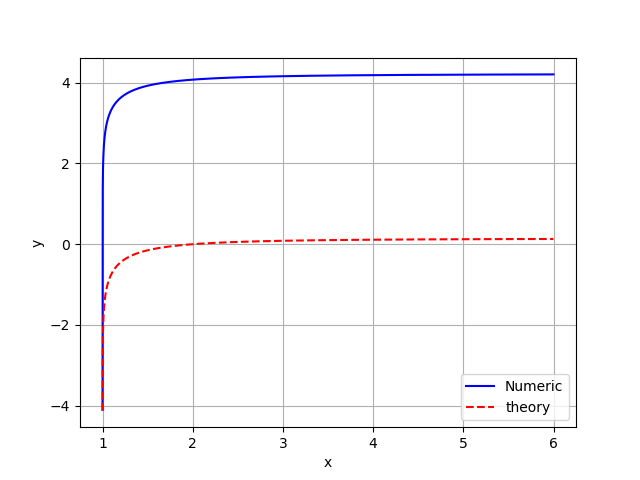
\includegraphics[width=0.7\linewidth]{figs/Figure_2.png}
   \label{Graph by Finite difference Method}
\end{figure}
\textbf{Note}:- Finite difference method fails here because $\frac{dy}{dx}$ is too large near x=1.Which creates a significant error in calculating $y_{n+1}$
\end{frame}

\section{Runga-kutta Method}
\subsection{Runga-kutta Method}
\begin{frame}
\frametitle{Runga-kutta Method}

Let ,
\begin{align} 
	h=0.001 \\
	\frac{dy}{dx} = f\brak{x_n} \\
\end{align}
Then ,
\begin{align} 
	k_1 = hf\brak{x_n}\\
	k_2 = hf\brak{x_n + h/2}\\
	k_3 = hf\brak{x_n + h/2}\\
	k_4 = hf\brak{x_n + h}\\
	k = \frac{1}{6}\brak{k_1 + 2k_2 + 2k_3+k_4}\\
	y_{n+1} = y_n + k\\
	x_{n+1} = x_{n} + h 
\end{align}
\end{frame}


\section{Plot by Runga-Kutta Method}
\subsection{Plot by Runga-Kutta Method}
\begin{frame}
\frametitle{Plot by Runga-Kutta Method}

\begin{figure}[h!]
   \centering
   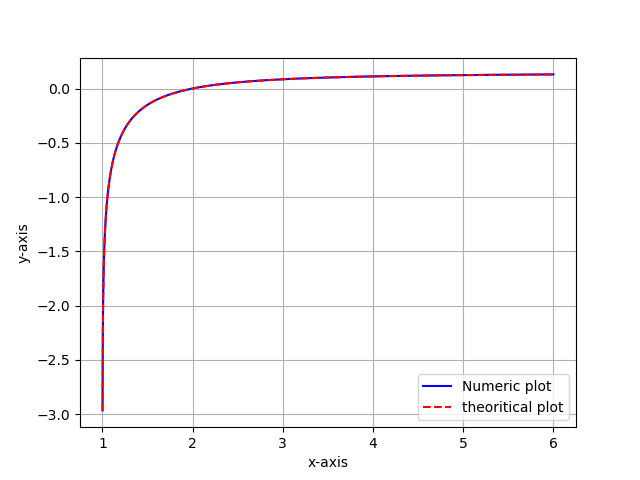
\includegraphics[width=0.7\linewidth]{figs/Figure_1.png}
   \label{Graph by Runga-Kutta Method}
\end{figure}
   

\end{frame}



\end{document}
